
\section{Physical Maps}
\label{sec-1}
Brazil\footnote{\url{http://en.wikipedia.org/wiki/Brazil}}, the world's fifth largest country, is one of the
seventeen megadiverse countries\footnote{\url{http://en.wikipedia.org/wiki/Megadiverse_countries}}, home to diverse wildlife,
natural environments, and extensive natural resources in a variety of
protected habitats. Throughout this section we will create a physical
map of this exceptional country using data from several data services.

\index{Packages!raster@\texttt{raster}}  
\index{Packages!rasterVis@\texttt{rasterVis}}  
\index{Packages!sp@\texttt{sp}}  
\index{Packages!maptools@\texttt{maptools}}  
\index{Packages!rgeos@\texttt{rgeos}}  
\index{Packages!colorspace@\texttt{colorspace}}  
\index{CRS@\texttt{CRS}}

\lstset{language=R,numbers=none}
\begin{lstlisting}
library(raster)
library(rasterVis)
library(maptools)
library(rgeos)
library(latticeExtra)
library(colorspace)

## Longitude-Latitude projection
proj <- CRS(' +proj=longlat +ellps=WGS84')
\end{lstlisting}

\subsection{Retrieving Data}
\label{sec-1-1}
Four types of information are needed: administrative boundaries,
terrain elevation, rivers and lakes, and sea depth.

\index{download.file@\texttt{download.file}}
\index{readShapePoly@\texttt{readShapePoly}}
\index{readShapeLines@\texttt{readShapeLines}}
\index{Encoding@\texttt{Encoding}}
\index{raster@\texttt{raster}}
\index{Data!GADM}
\index{Data!DIVA-GIS}
\index{Data!Natural Earth Data}

\begin{enumerate}
\item The administrative boundaries are available from GADM\footnote{\url{http://gadm.org/}}. The
\texttt{readShapePoly} function reads data from the downloaded shapefile
and creates a \texttt{SpatialPolygonsDataFrame} object.
\lstset{language=R,numbers=none}
\begin{lstlisting}
old <- setwd(tempdir())

download.file('http://www.gadm.org/data/shp/BRA_adm.zip',
	      'BRA_adm.zip')
unzip('BRA_adm.zip')
brazilAdm <- readShapePoly('BRA_adm1.shp', proj4string=proj)
Encoding(levels(brazilAdm$NAME_1)) <- 'latin1'
\end{lstlisting}

\item The terrain elevation or digital elevation model (DEM) is
available from DIVA-GIS\footnote{\url{http://www.diva-gis.org/Data}}. The \texttt{raster} function reads the
file and creates a \texttt{RasterLayer} object.
\lstset{language=R,numbers=none}
\begin{lstlisting}
download.file('http://www.diva-gis.org/data/alt/BRA_alt.zip',
	      'BRA_alt.zip')
unzip('BRA_alt.zip')
brazilDEM <- raster('BRA_alt')
\end{lstlisting}
\item The water lines (rivers and lakes) are available from Natural
Earth Data\footnote{\url{http://www.naturalearthdata.com/}}. The \texttt{readShapeLines} function reads data from
the downloaded shapefile and creates a \texttt{SpatialLinesDataFrame}
object.
\lstset{language=R,numbers=none}
\begin{lstlisting}
## World Water lines (Natural Earth)
download.file('http://www.naturalearthdata.com/http//www.naturalearthdata.com/download/10m/physical/ne_10m_rivers_lake_centerlines.zip',
	      'neRivers.zip')
unzip('neRivers.zip')
worldlRiv <- readShapeLines('ne_10m_rivers_lake_centerlines', proj4string = proj)
\end{lstlisting}
\item Finally, the sea depth is also available from Natural Earth
Data\footnotemark[5]{}. The raster covers the whole world so it must be
cropped by the extent of the DEM raster.
\lstset{language=R,numbers=none}
\begin{lstlisting}
download.file('http://www.naturalearthdata.com/http//www.naturalearthdata.com/download/10m/raster/OB_LR.zip',
	      'neSea.zip')
unzip('neSea.zip')
worldSea <- raster('OB_LR.tif')
brazilSea <- crop(worldSea, brazilDEM)
setwd(old)
\end{lstlisting}
\end{enumerate}
\subsection{Intersection of Shapefiles and Elevation Model}
\label{sec-1-2}
The rivers and lakes database from Natural Earth Data comprises all
the world extent, but we only need the rivers of Brazil. The function
\texttt{gIntersection} of the package \texttt{rgeos} determines the intersection
between two geometries. Because these geometries must be defined with
classes of the \texttt{sp} package, the extent of \texttt{brazilDEM} must be first
converted to \texttt{SpatialPolygons}. The intersection is a new
\texttt{SpatialLines} object, \texttt{brazilRiv}.

\index{gIntersection@\texttt{gIntersection}}
\index{extent@\texttt{extent}}

\lstset{language=R,numbers=none}
\begin{lstlisting}
## only those features labeled as "River" are needed
worlRiv<- worlRiv[worlRiv$featurecla=='River',]

## Define the extent of Brazil as a SpatialPolygons
extBrazil <- as(extent(brazilDEM), 'SpatialPolygons')
proj4string(extBrazil) <- proj

## and intersect it with worldRiv to extract brazilian rivers
## from the world database
brazilRiv <- gIntersection(worldRiv, extBrazil, byid=TRUE)
## and especially the famous Amazonas River
amazonas <- worldRiv[worldRiv$name=='Amazonas',]
\end{lstlisting}
\subsection{Labels}
\label{sec-1-3}
Each region of Brazil will be labeled with the name of its
corresponding polygon. The locations of the labels are defined by the
centroid of each polygon, easily computed with the \texttt{coordinates}
method. In addition, a larger label with the name of the country will be
placed in the average centroid.

\index{coordinates@\texttt{coordinates}}
\index{apply@\texttt{apply}}

\lstset{language=R,numbers=none}
\begin{lstlisting}
## Locations of labels of each polygon
centroids <- coordinates(brazilAdm)
## Location of the "Brazil" label (average of the set of polygons centroids)
xyBrazil <- apply(centroids, 2, mean)
\end{lstlisting}

Some region names are too long to be displayed in one line. Thus, a
previous step is to split the string if it comprises more than two
words.

\index{sapply@\texttt{sapply}}
\index{strsplit@\texttt{strsplit}}

\lstset{language=R,numbers=none}
\begin{lstlisting}
admNames <- strsplit(as.character(brazilAdm$NAME_1), ' ')

admNames <- sapply(admNames,
		 FUN=function(s){
		   sep=if (length(s)>2) '\n' else  ' '
		   paste(s, collapse=sep)
		   })
\end{lstlisting}
\subsection{Overlaying Layers of Information}
\label{sec-1-4}
Therefore, the physical map (Figure \ref{fig:brazil}) is composed
of four layers: 

\begin{enumerate}
\item The sea depth raster displayed with the \texttt{levelplot} method of the
\texttt{rasterVis} package. The palette is defined with \texttt{brewer.pal}
(Figure \ref{fig:rastersBrazil}).
\lstset{language=R,numbers=none}
\begin{lstlisting}
blueTheme <- rasterTheme(region=brewer.pal(n=9, 'Blues'))

seaPlot <- levelplot(brazilSea, par.settings=blueTheme,
		    maxpixels=1e6, panel=panel.levelplot.raster,
		    margin=FALSE, colorkey=FALSE)
\end{lstlisting}

\index{rasterTheme@\texttt{rasterTheme}}
\index{brewer.pal@\texttt{brewer.pal}}

\item The altitude raster layer uses a terrain colors palette, as the one
produced by the \texttt{terrain\_hcl} function from the \texttt{colorspace} package
\cite{Ihaka.Murrell.ea2011} (Figure \ref{fig:rastersBrazil}).
\lstset{language=R,numbers=none}
\begin{lstlisting}
terrainTheme <- rasterTheme(region=terrain_hcl(15))

altPlot <- levelplot(brazilDEM, par.settings=terrainTheme,
		     maxpixels=1e6, panel=panel.levelplot.raster,
		     margin=FALSE, colorkey=FALSE)
\end{lstlisting}

\index{rasterTheme@\texttt{rasterTheme}}
\index{terrain_hcl@\texttt{terrain\_hcl}}

\item The rivers represented by the \texttt{SpatialLinesDataFrame} object. The
Amazonas River is labeled with \texttt{sp.lineLabel} and printed with a
thicker line. The label is created with the \texttt{label} method, a
wrapper function to extract the \texttt{ID} slots from the \texttt{SpatialLines}
and create a suitable \texttt{character} object with the correct \texttt{names}
values.

\lstset{language=R,numbers=none}
\begin{lstlisting}
amazonasLab <- label(amazonas, 'Amazonas')
\end{lstlisting}

\item The administrative boundaries represented by the
\texttt{SpatialPolygonsDataFrame} object with their labels printed with
the \texttt{panel.pointLabel} function. This function uses optimization
routines to find good locations for point labels without overlaps.

\index{levelplot@\texttt{levelplot}}
\index{sp.lines@\texttt{sp.lines}}
\index{sp.lineLabel@\texttt{sp.lineLabel}}
\index{sp.polygons@\texttt{sp.polygons}}
\index{panel.text@\texttt{panel.text}}
\index{layer@\texttt{layer}}
\index{brewer.pal@\texttt{brewer.pal}}

\lstset{language=R,numbers=none}
\begin{lstlisting}
 seaPlot + altPlot + layer({
    ## Rivers
    sp.lines(brazilRiv, col='darkblue', lwd=0.2)
    ## Amazonas
    sp.lineLabel(amazonas, amazonasLab, 
		 lwd=1, col='darkblue', col.line='darkblue',
		 cex=0.5, fontfamily='Palatino')
    ## Administrative boundaries
    sp.polygons(brazilAdm, col='black', lwd=0.2)
    ## Centroids of administrative boundaries ...
    panel.points(centroids, col='black')
    ## ... with their labels
    panel.pointLabel(centroids, labels=admNames,
		     cex=0.7, fontfamily='Palatino', lineheight=.8)
    ## Country name
    panel.text(xyBrazil[1], xyBrazil[2], labels='B R A Z I L',
	       cex=1.5, fontfamily = 'Palatino', fontface=2)
})
\end{lstlisting}
\end{enumerate}

\begin{figure}[htb]
\centering
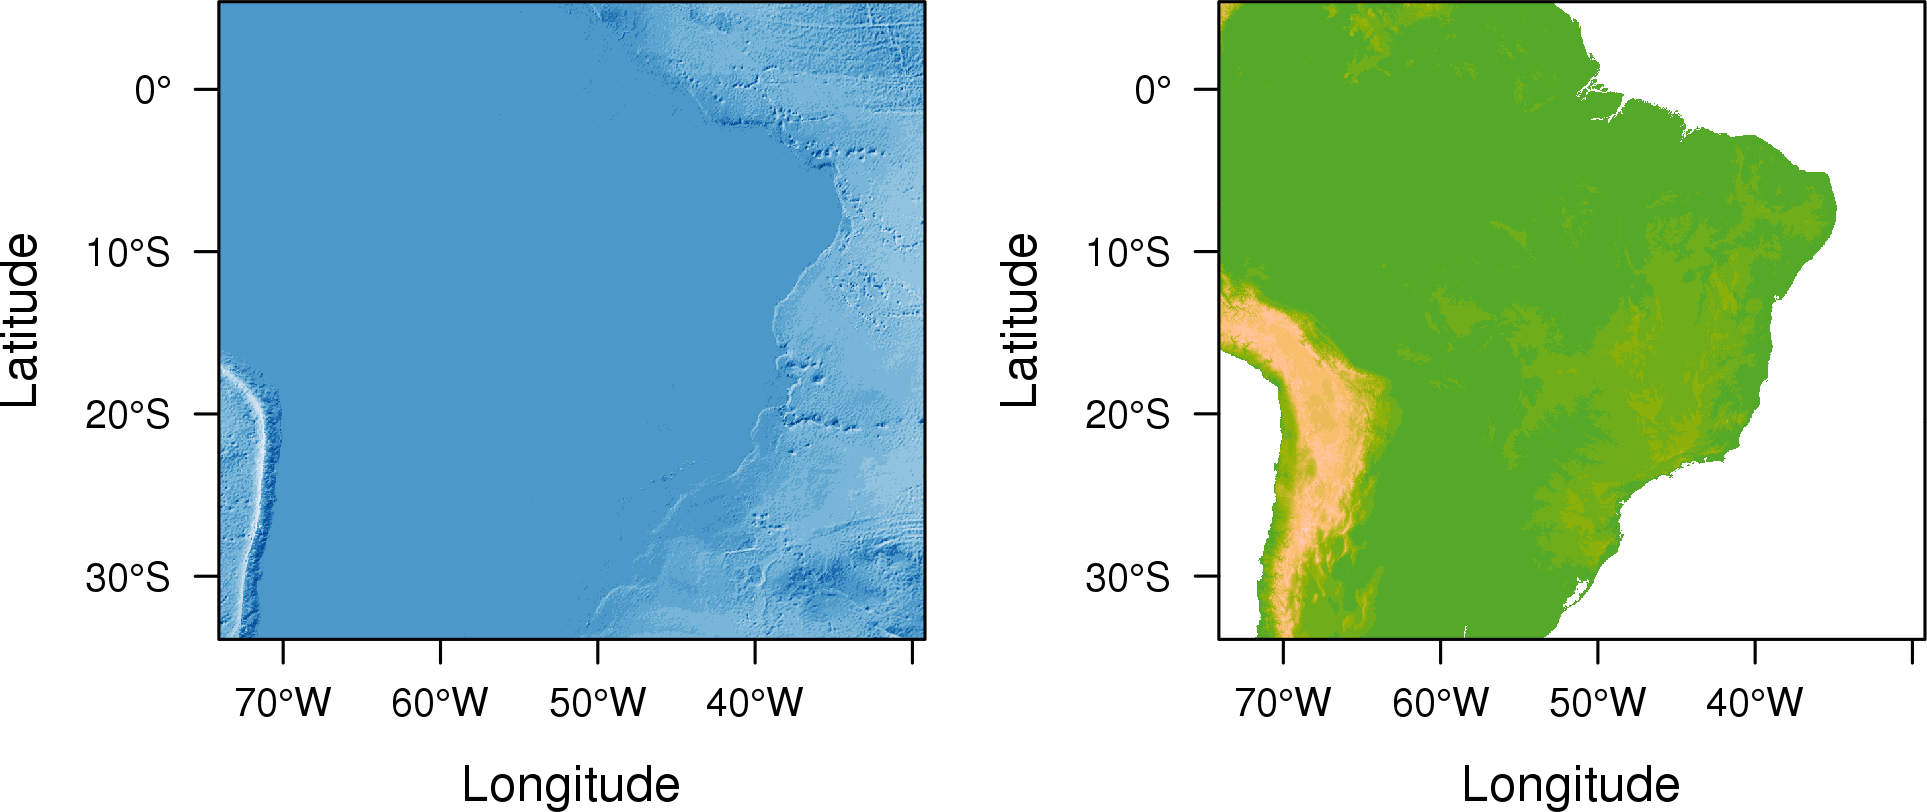
\includegraphics[width=.9\linewidth]{figs/rastersBrazil.png}
\caption{\label{fig:rastersBrazil}Sea depth and altitude rasters of Brazil.}
\end{figure}


\begin{figure}[htb]
\centering
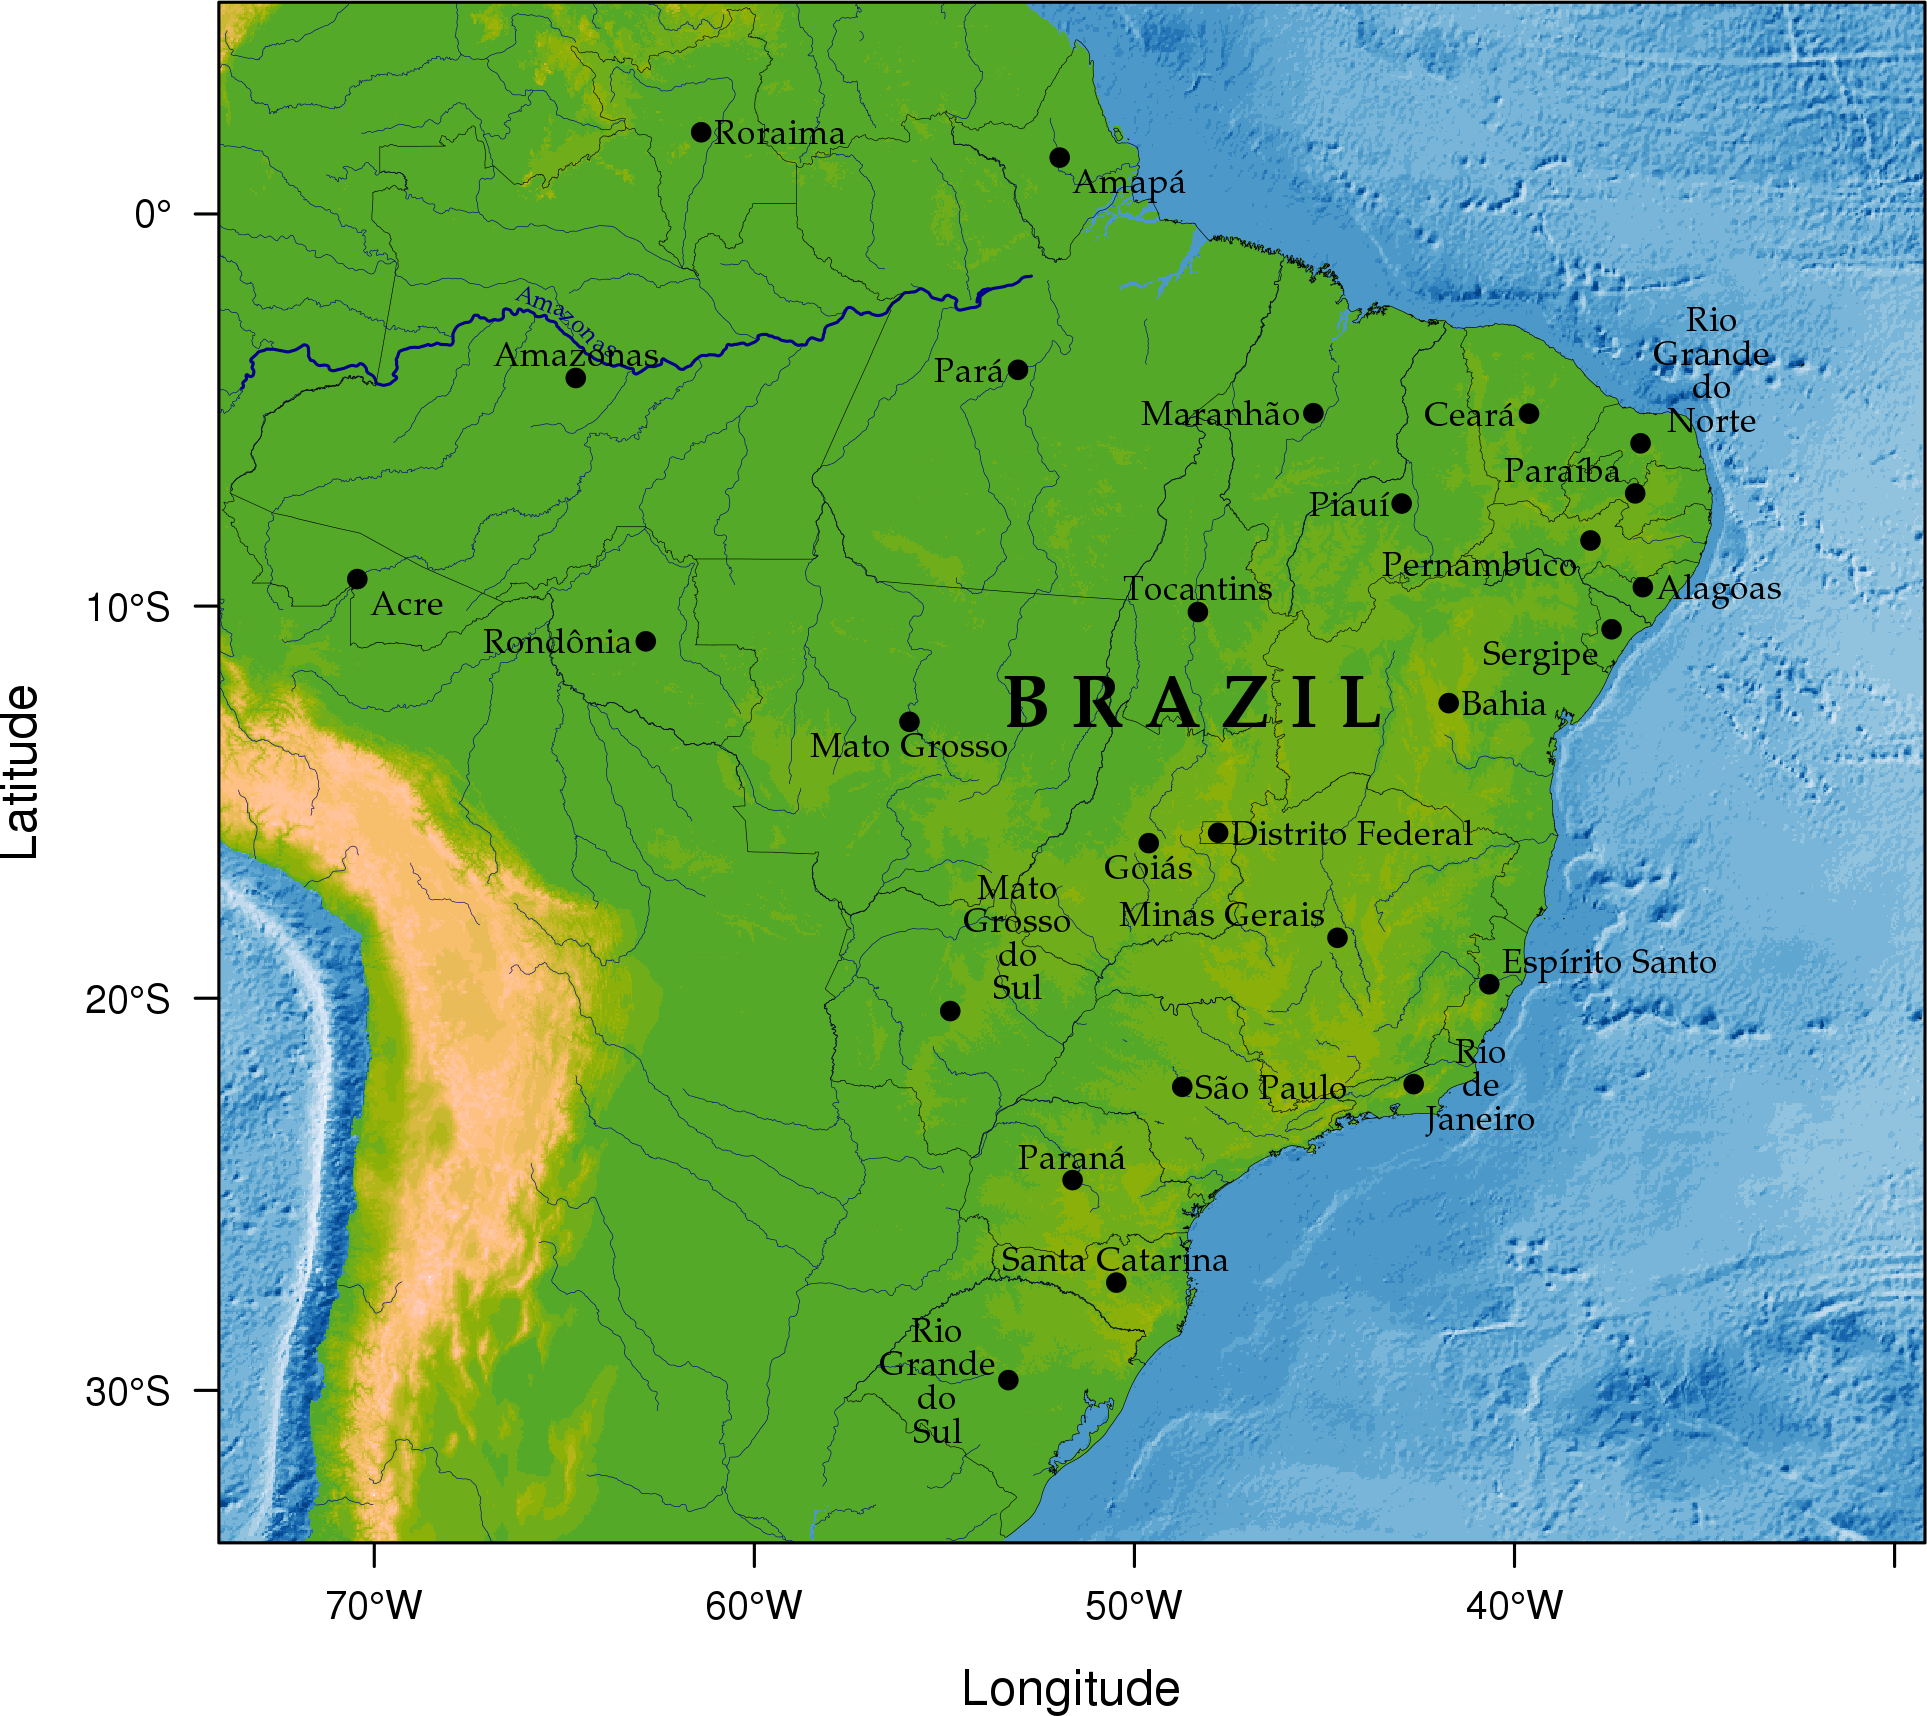
\includegraphics[width=.9\linewidth]{figs/brazil.png}
\caption{\label{fig:brazil}Physical map of Brazil. Main administrative regions and the Amazonas River are labeled.}
\end{figure}
